\paragraph{Sơ đồ tuần tự luồng nhắn tin văn bản qua SSE}

Luồng nghiệp vụ này mô tả
vòng đời của một
yêu cầu chat văn bản từ Web Frontend tới Conversation Service,
qua Chatbot Service bằng gRPC streaming
và trả kết quả về client bằng Server-Sent Events (SSE).
Luồng bao gồm kiểm tra quyền VIP khi bật reasoning,
truyền token qua gRPC metadata,
stream các thông tin \texttt{status}, \texttt{content}, \texttt{metadata}, đồng thời lưu lịch sử chat ở Chatbot Service.

\begin{figure}[H]
\centering
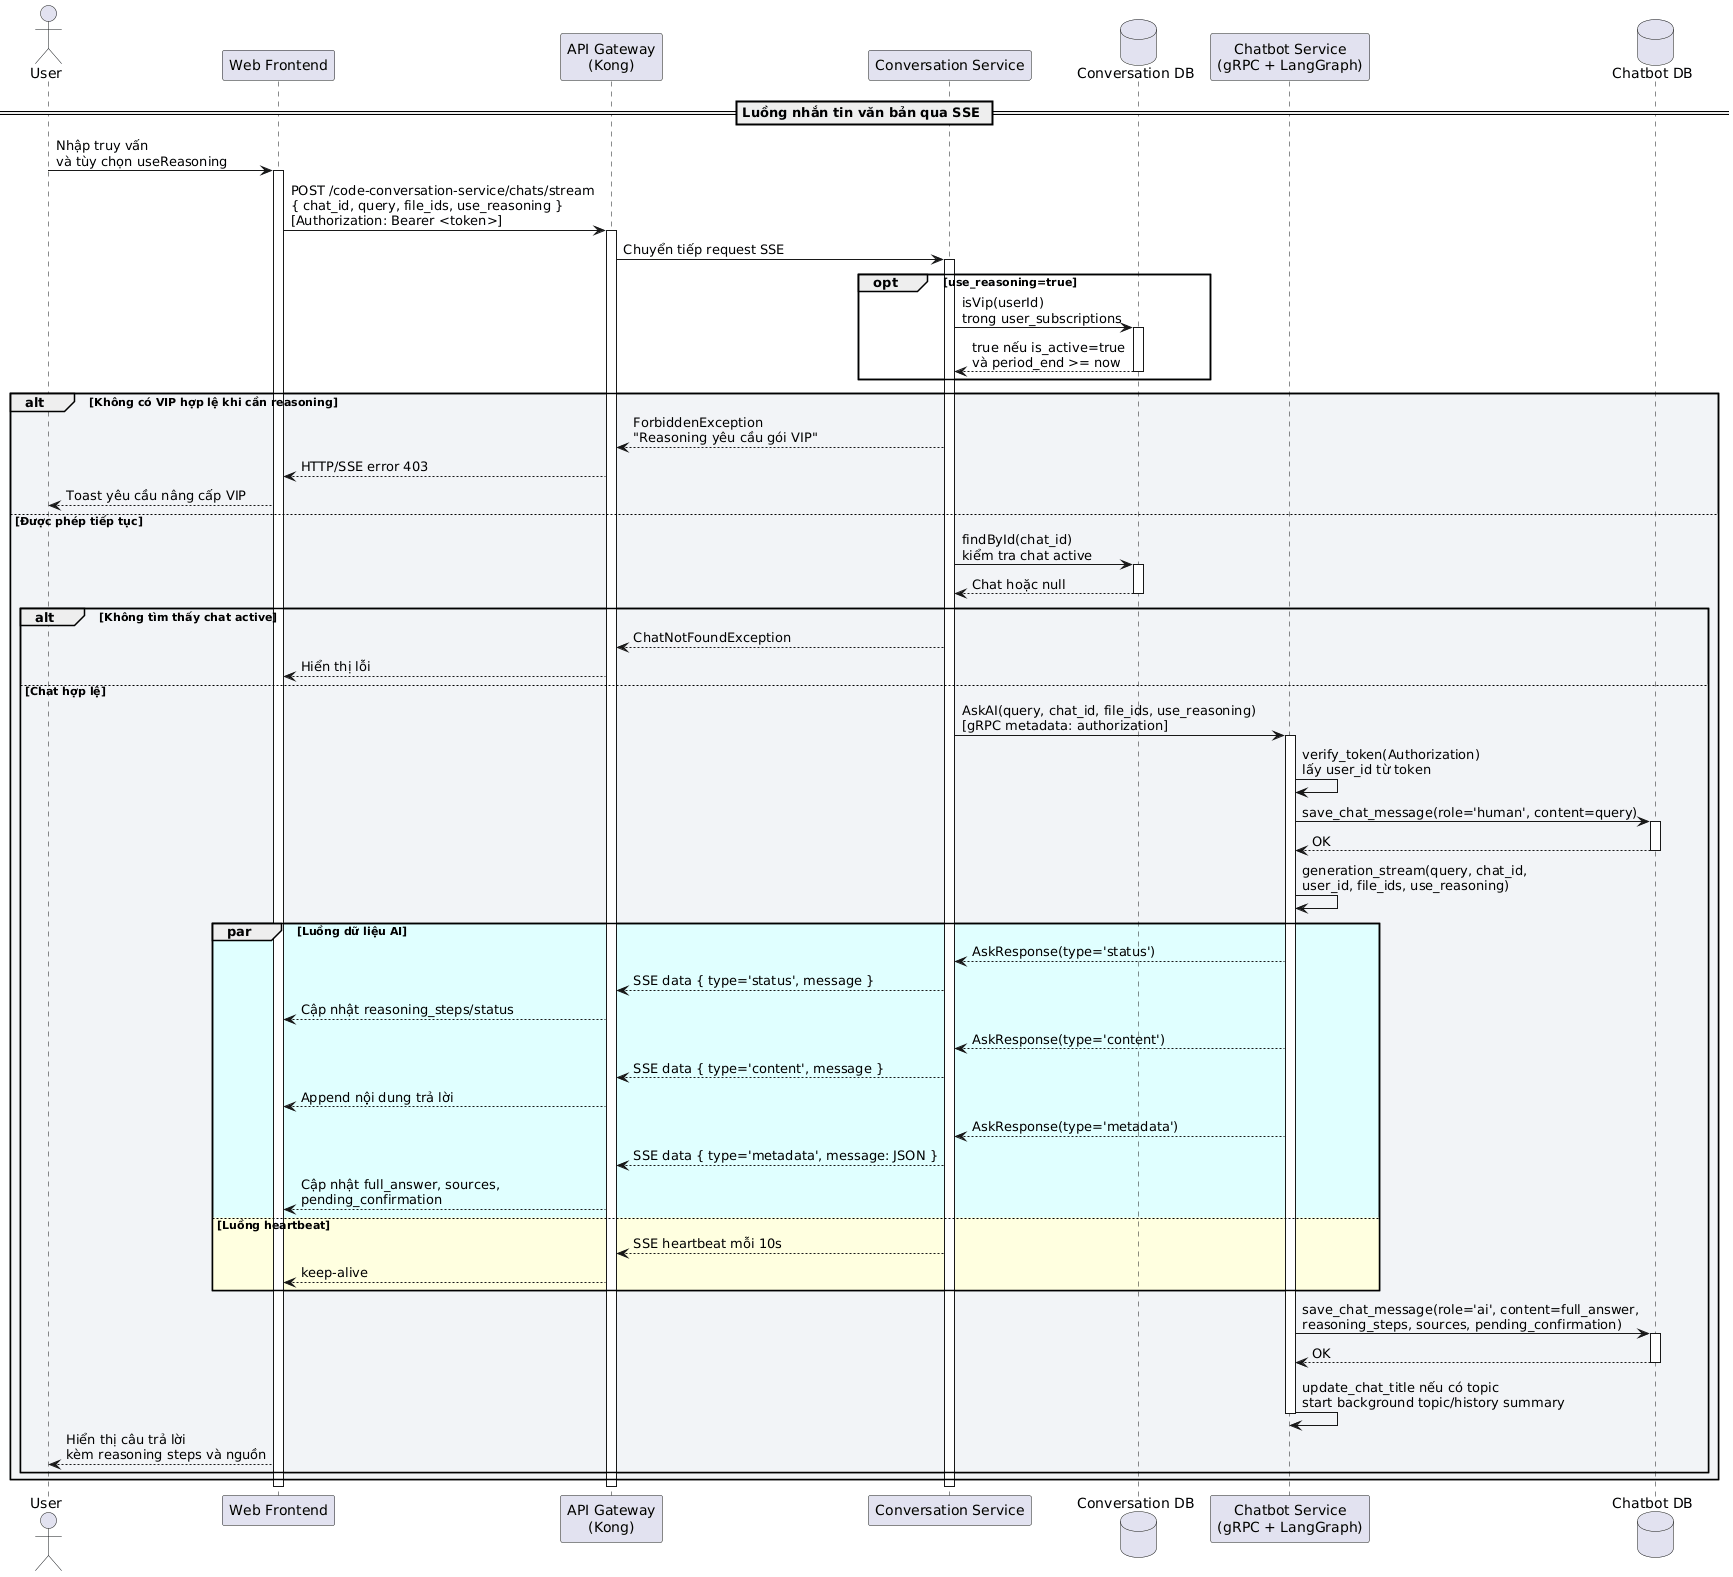
\includegraphics[width=0.95\textwidth]{contents/Sequence/UML-Sequence-UserTextChatSse.png}
\caption{Sơ đồ tuần tự luồng nhắn tin văn bản qua SSE}
\end{figure}

\subparagraph{Mô tả tổng quan}

\begin{itemize}

\item \textbf{Gửi yêu cầu trò chuyện:}
Giao diện gửi yêu cầu trò chuyện
truyền dữ liệu liên tục
kèm định danh cuộc trò chuyện, nội dung câu hỏi, danh sách tài liệu chọn phân tích, tùy chọn sử dụng lập luận nâng cao và mã đăng nhập qua cổng API.

\item \textbf{Kiểm tra quyền hạn:}
Dịch vụ trò chuyện nhận yêu cầu:
nếu người dùng muốn sử dụng lập luận nâng cao, dịch vụ kiểm tra trạng thái gói thuê bao VIP của người dùng trong CSDL xem có đang hoạt động
và còn thời hạn hay không. Nếu không hợp lệ sẽ trả về lỗi từ chối quyền truy cập.

\item \textbf{Kiểm tra cuộc trò chuyện:}
Dịch vụ trò chuyện
kiểm tra định danh cuộc trò chuyện
để đảm bảo cuộc trò chuyện còn tồn tại và đang hoạt động. Nếu không tìm thấy sẽ trả về thông báo lỗi.

\item \textbf{Kết nối dịch vụ chatbot:}
Dịch vụ trò chuyện
gọi dịch vụ chatbot
và chuyển tiếp thông tin cuộc trò chuyện.

\item \textbf{Truyền dữ liệu trực tiếp:}
Dịch vụ chatbot
kiểm tra thông tin, lưu tin nhắn của người dùng vào CSDL chatbot,
sau đó truyền trực tiếp
từng phân đoạn kết quả câu trả lời về cho dịch vụ trò chuyện.

\item \textbf{Lưu lịch sử và lập luận:}
Khi hoàn thành câu trả lời cuối cùng,
dịch vụ chatbot
lưu câu trả lời của hệ thống cùng các bước lập luận, nguồn tài liệu tham khảo
và trạng thái chờ xác nhận vào CSDL chatbot,
đồng thời cập nhật chủ đề cuộc trò chuyện
hoặc chạy công việc tóm tắt nội dung cuộc trò chuyện trong nền nếu cần.

\end{itemize}

\begin{table}[H]
\centering
\renewcommand{\arraystretch}{1.3}

\begin{tabular}{|l|l|p{5cm}|}
\hline
\textbf{Thành phần} & \textbf{Phân loại} & \textbf{Vai trò trong hệ thống} \\ \hline
User & Actor & Người dùng nhập truy vấn, chọn tài liệu đính kèm và tùy chọn bật reasoning. \\ \hline
Web Frontend & Component & Giao diện web Next.js. \\ \hline
API Gateway (Kong) & Component & Cổng API chuyển tiếp các yêu cầu API. \\ \hline
Conversation Service & Microservice & Kiểm tra quyền VIP khi cần, kiểm tra chat active, mở SSE stream và gọi Chatbot Service qua gRPC. \\ \hline
Conversation DB & Database & Lưu quản lý trò chuyện và và bảng \texttt{user\_subscriptions} dùng để kiểm tra VIP. \\ \hline
Chatbot Service (gRPC + LangGraph) & Microservice & Verify token từ gRPC metadata, xử lý RAG/reasoning, stream kết quả và lưu lịch sử chat. \\ \hline
Chatbot DB & Database & Lưu human message, AI message, reasoning steps, sources và trạng thái xác nhận. \\ \hline
\end{tabular}
\caption{Các thành phần tham gia luồng nhắn tin văn bản qua SSE}
\end{table}
